%This section delves into how the transformer was implemented and tuned for the given task.
\subsubsection{Motivation}
In the past few years, transformers have risen in popularity in the NLP space. 
Student summaries have mostly long sequence lengths and require an efficient and capable architecture to fit the data.
Transformers are a perfect fit for the challenge at hand.

\subsubsection{Transformer selection}
When choosing the most fitting and optimal transformer multiple factors must be taken into consideration.
This would be the type of transformer for instance or how the attention mechanism was implemented.
Nevertheless, from just observing the desired result, which is predicting two continuous values, several factors can already be decided on.
Encoder-only models were chosen because there is no need for decoders, as there is nothing to decode.
From that observation, the team searched for suitable models on HuggingFace\footnote{\href{https://huggingface.co/}{HuggingFace - Website}}, a platform listing various transformer implementations. The search focused on encoder-only models, sorted by popularity.
Additionally, the complexity of the transformers was considered, along with trials of both uncased and cased models to assess their impact on performance.
All tested implementations were variations of BERT, primarily due to the team's limited familiarity and expertise with non-BERT-based models.\\

\noindent The best performing implementation was found as follows:
Since the public data only consists of four possible topics and the private data set of an unknown number of topics, a great importance on generalization was set.
Due to this, the cross-validation technique Group-K Fold was used. With this method the generalization performance can be estimated on unseen topics.
The models are trained on the training set using the HuggingFace Transformers library and the \gls{rmse} of the content and wording score, and the combination of \gls{mcrmse} were used to compute the metrics:

\vspace{1em}

\begin{lstlisting}
def compute_mcrmse(eval_pred):
    preds, labels = eval_pred

    col_rmse = np.sqrt(np.mean((preds - labels) ** 2, axis=0))
    mcrmse = np.mean(col_rmse)

    return {
        "content_rmse": col_rmse[0],
        "wording_rmse": col_rmse[1],
        "mcrmse": mcrmse,
    }
\end{lstlisting}

\vspace{2em}

\noindent When running the test all models had the exact same hyperparameter configuration:%. The following hyperparameters were used:
\begin{itemize}
	\item \textbf{Input:} The tokenized padded or truncated student-written summary.
	\item \textbf{\gls{max_length}:} 512. This was chosen since most of the BERT models have 512 as maximum length.
	\item \textbf{\gls{batch_size}:} 8
    \item \textbf{\glspl{epoch}:} 8
    \item \textbf{\gls{lr}:} 0.0001
    \item \textbf{\gls{weight_decay}:} 0.01
\end{itemize}
\textbf{NOTE:} Hyperparameters which are not listed above use the default settings from the HuggingFace Library.

\begin{figure}[H]
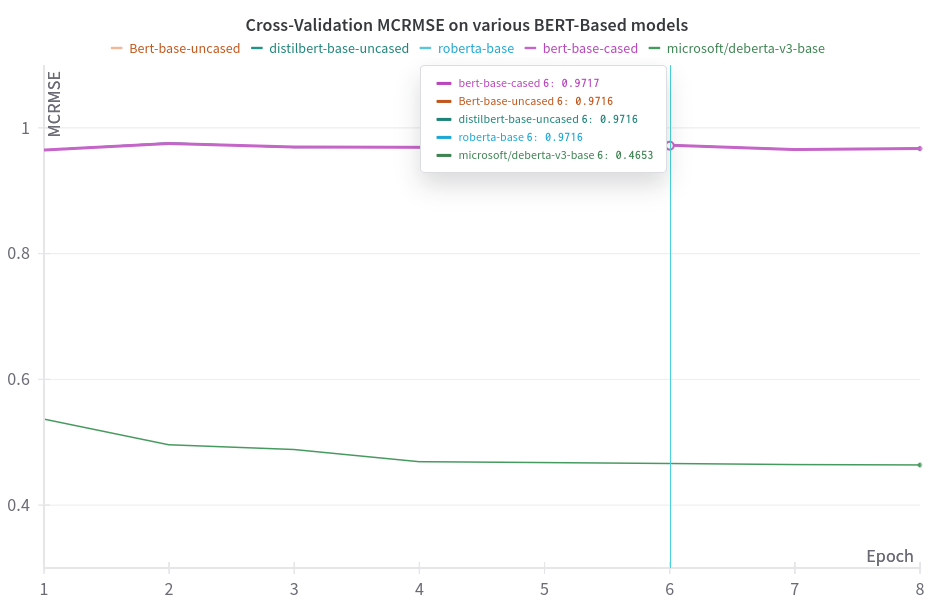
\includegraphics[keepaspectratio, width=\textwidth]{img/cross-validation-performance.png}
\caption{Cross-Validation MCRMSE Score Evolution on various BERT-Based models}
\label{fig:cross-validation}
\end{figure}
\vspace{1em}

The above visualization distinctly highlights a standout performer. All BERT-based models, except for DeBERTa fail to generalize effectively.
It is noteworthy that the performance metrics of models other than DeBERTa are quite similar, suggesting minimal variance among them. Additionally, the comparison of uncased and cased BERT-based models indicates that the casing does not significantly influence performance outcomes.
A possible reason for DeBERTa outperforming, and also what it makes it different compared to the other BERT-Based models, is the disentangled attention mechanism.

\subsubsection{Prompt Engineering}
When using transformers, using an optimized prompt has been proven to achieve better results.
Various experiments using different combinations of features from the data were conducted.
A logical combination of the features would be to use the student-written text together with the prompt text.
After further experimenting, adding the prompt question and using a natural language style prompt improved performance.

\begin{figure}[H]
\begin{center}
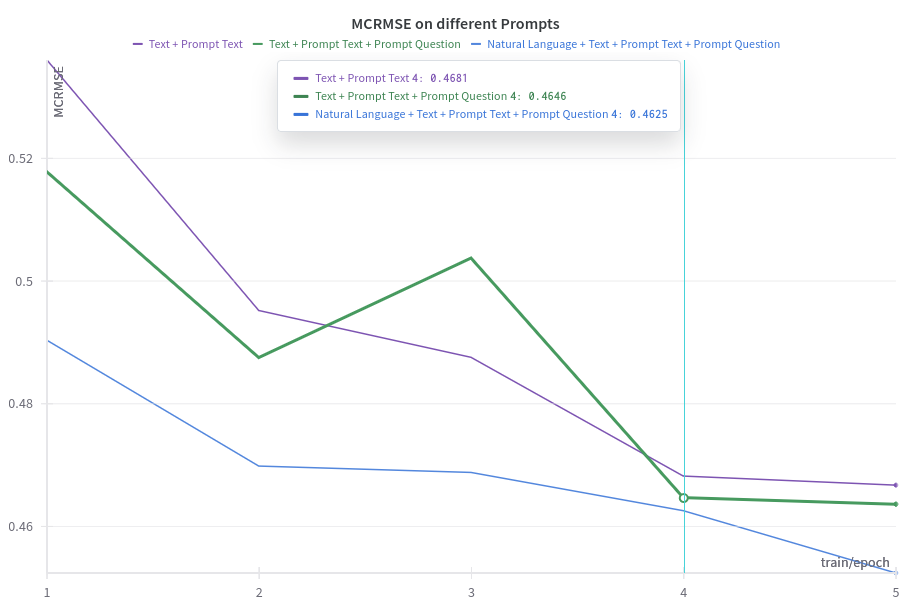
\includegraphics[keepaspectratio, width=\textwidth]{img/prompts.png}
\caption{MCRMSE Score Evolution on different Prompts}
\label{fig:prompts}
\end{center}
\end{figure}

\vspace{1em}

By using a natural language style prompt, verbs and objectives were used to specify the goal of the problem at hand.
The final prompt the transformer uses is the following:

\begin{quote}
    ``Evaluate the content and wording score of this summary: [SEP] \textbf{text} [SEP] The summary must answer the following prompt: [SEP] \textbf{prompt question} [SEP] The prompt is related towards the following original text: [SEP] \textbf{prompt text}''
\end{quote}

\subsubsection{Model Architecture}
The model uses three features from the dataset which are the student-written summary, the prompt text, and the prompt question.
These get formatted into the aforementioned prompt and \glsdisp{token}{tokenized}. The tokenizer pads or truncates the prompt to the max length.
The network then outputs the content and wording scores for the summary.

\begin{figure}[H]
\begin{center}
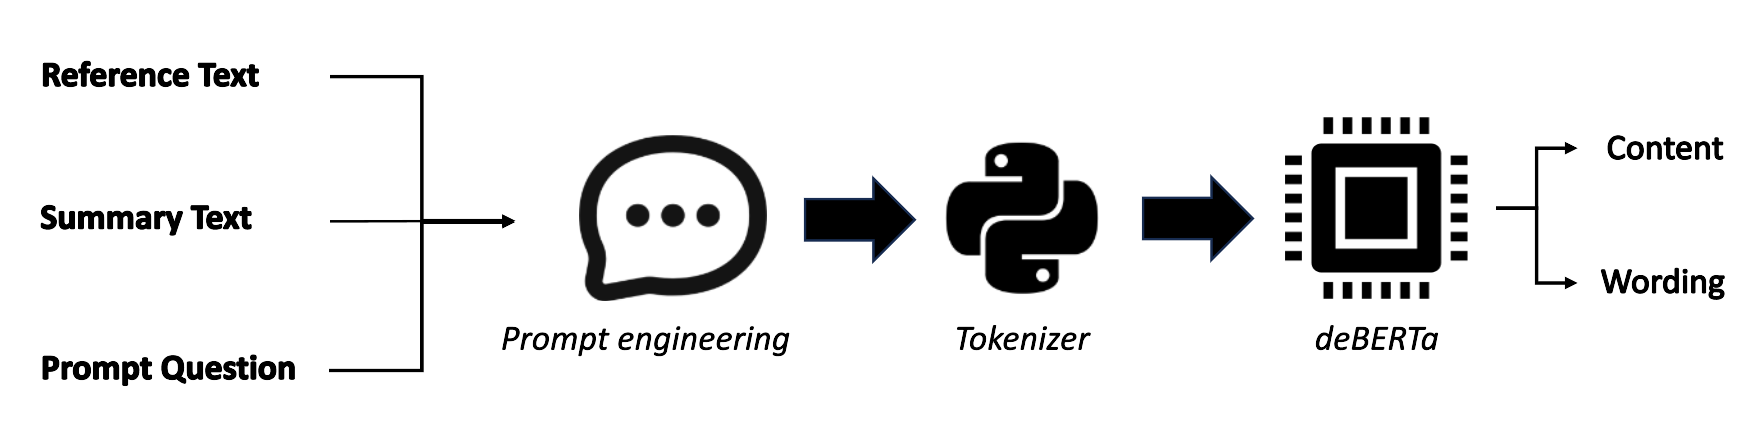
\includegraphics[keepaspectratio, width=0.8\textwidth]{img/transformer_architecture.png}
\caption{Transformer Pipeline}
\label{fig:transformer_architecture}
\end{center}
\end{figure}
\subsubsection{Hyperparameter tuning}
\subsubsection*{Layer fine-tuning}
DeBERTa contains twelve encoding layers. The Transformer model was downstreamed by freezing the bottom N layers.
After iterating and freezing each layer, the best performing iteration was freezing at layer 9:

\begin{figure}[H]
\begin{center}
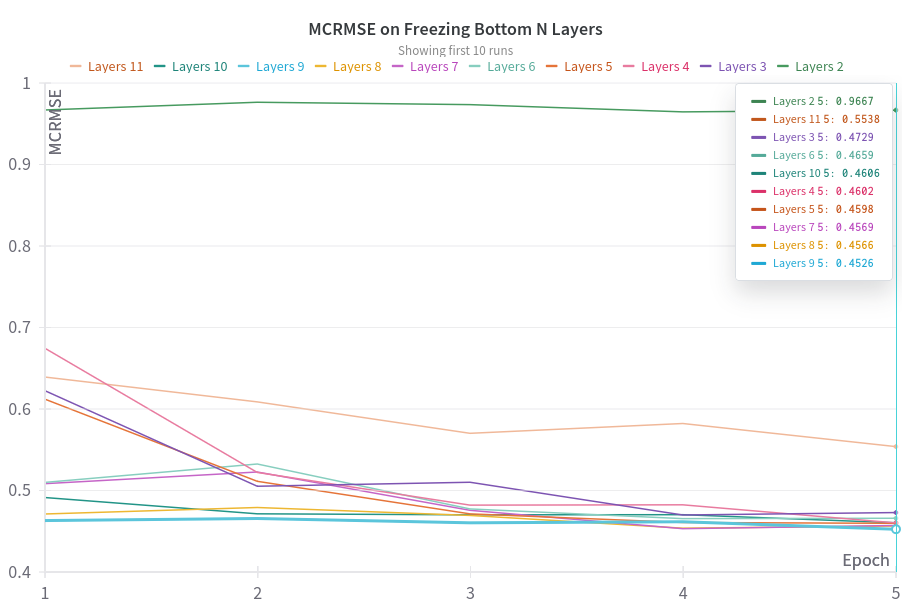
\includegraphics[keepaspectratio, width=0.86\textwidth]{img/n_layers.png}
\caption{MCRMSE Score Evolution on freezing N Layers}
\label{fig:n_layers}
\end{center}
\end{figure}
\subsubsection*{Max length fine-tuning}
Configuring the max length was essential, because if the max length is too short it could cut out important information of the prompt.
A logical conclusion would be that a higher max length would lead to better performance. However, sequence lengths over 1024 led to worse performance.
It is speculated that the text of the prompt exceeding 1024 \glspl{token} may become overly detailed, potentially impacting the results negatively.

\begin{figure}[H]
\begin{center}
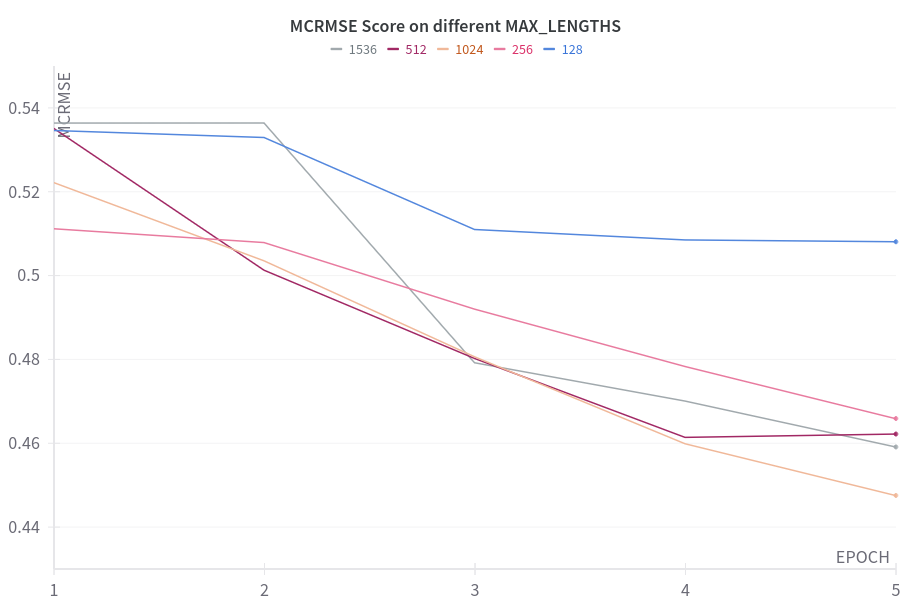
\includegraphics[keepaspectratio, width=0.9\textwidth]{img/max_length.png}
\caption{MCRMSE Score Evolution on different Max Lengths}
\label{fig:max_length}
\end{center}
\end{figure}

\subsubsection*{Hyperparameter configuration}
Below are the hyperparameters that were tuned and an explanation why the specific values were chosen.

\begin{itemize}
	\item \textbf{Max length:} 1024. Best performing max length.
	\item \textbf{Batch size:} 4. Maximum allowed batch size due to hardware limitation.
    \item \textbf{Epochs:} 4. MCRMSE Score converges at four epochs. Also, having too many epochs could lead to overfitting.
    \item \textbf{Learning rate:} 0.0001. Automatically fine-tuned using optuna\footnote{\href{https://optuna.org/}{Optuna - Automatic Hyperparameter Optimizer}}.
    \item \textbf{Weight decay:} 0.01. Automatically fine-tuned using optuna.
    \item \textbf{Hidden dropout prob:} 0.07. Automatically fine-tuned using optuna.
    \item \textbf{Attention probs dropout prob:} 0.07. Automatically fine-tuned using optuna.
\end{itemize}
\textbf{NOTE:} Hyperparameters which are not listed above use the default settings from the HuggingFace Library.


\subsubsection{Transformer result}
As seen in Figure~\ref{fig:deberta_performance}, the performance on the content score is high. However, improvements can be made on the wording score.

\begin{figure}[H]
    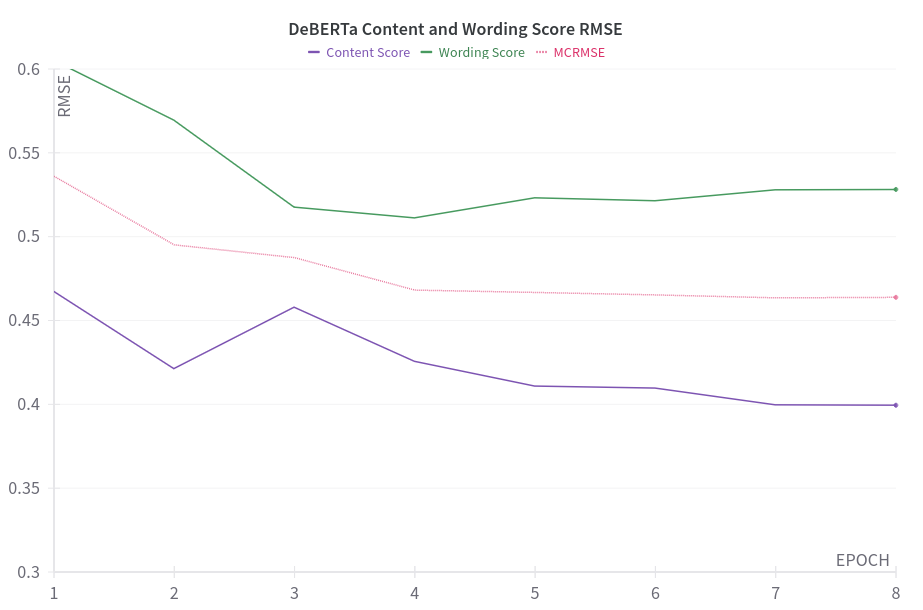
\includegraphics[keepaspectratio, width=\textwidth]{img/Deberta-performance.png}
\caption{Deberta Performance on Wording and Content}
\label{fig:deberta_performance}
\end{figure}